\documentclass[12pt]{article}
\usepackage{amssymb, amsmath}
\usepackage{bm}
\usepackage{dsfont}
\usepackage{empheq}
\usepackage{graphicx}
\usepackage{float}
\usepackage{xcolor,cancel}

% Set up the margins.
\usepackage[top=1in, bottom=1in, left=1in, right=1in]{geometry}

% See
%   https://tex.stackexchange.com/questions/20609/strikeout-in-math-mode/20612
%
\newcommand\hcancel[2][black]{\setbox0=\hbox{$#2$}
\rlap{\raisebox{.45\ht0}{\textcolor{#1}{\rule{\wd0}{1pt}}}}#2}

\begin{document}


\section{Probabilistic Graphical Models 1: Representation}

\subsection{Week 1. Introduction and Overview}

Please see the student example in Fig.~\ref{fig:student_example}.

\begin{figure}[H]
\centering
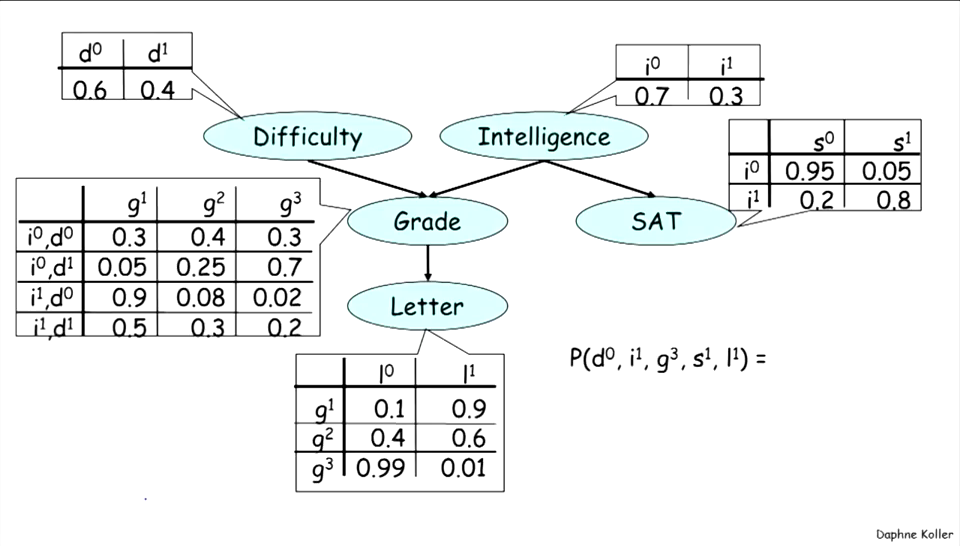
\includegraphics[width=6in]{graphics/example_student.png}
\caption{Student Example. Each node is annotated with a conditional probability distribution (CPD).}
\label{fig:student_example}
\end{figure}


\begin{itemize}
    \item Grade ($G$) --- $g^1(A)$, $g^2(B)$, and $g^3(C)$.
    \item Course Difficulty ($D$) --- $d^0(\text{easy})$, $d^1(\text{hard})$.
    \item Student Intelligence ($I$) --- $i^0(\text{low})$ and $i^1(\text{high})$.
    \item SAT score ($S$).
    \item Reference Letter ($L$).
\end{itemize}
 

% D, I --> G --> L
% I --> S


\subsubsection{Joint Distribution}
Consider $\Pr(I, D, G)$.

\subsubsection{Conditioning}
For example, we can condition on $G=g^1$.  We look at $\Pr(I, D, g^1)$.
We need to renormalize. That is
\begin{equation*}
  \Pr(I, D | g^1) = \frac{\Pr(I, D, g^1)}
                         {\sum_{I=i^j} \sum_{D=d^k} \Pr(I, D, g^1)}  \, .
\end{equation*}
The above equation comes from the definition of conditional probability $\Pr(A | B) = \Pr(A, B) / \Pr(B)$.

\subsubsection{Marginalization}
For example, we marginalize $I$.

\begin{equation*}
  \Pr(D) = \sum_{I=i^j} \Pr(I, D)
\end{equation*}


\subsubsection{Factors}
A factor $\phi$ maps random variables to a real number. That is
\begin{equation*}
  \phi : (X_1, \ldots, X_k) \rightarrow \Re
\end{equation*}
A joint distribution $\Pr(I, D, G)$ is a factor.

We compute a factor product using
\begin{equation*}
  \phi(A=a^i, B=b^j, C=c^k) = \phi_1(A=a^i, B=b^j) \phi_2(B=b^j, C=c^k) \, .
\end{equation*}

We can marginalize a factor too.
\begin{equation*}
  \phi(A=a^i, C=c^k) = \sum_j \phi(A=a^i, B=b^j, C=c^k) \,.
\end{equation*}




\subsection{Week 1. Bayesian Network (Directed Models)}

A Bayesian network is a directed acyclic graph (DAG) whose nodes represent the random variables $X_1, \ldots, X_n$.
\subsubsection{Factorization}
Chain rule:
\begin{equation}
  \Pr(D, I, G, S, L) = \Pr(D) \Pr(I) \Pr(G|I, D) \Pr(S|I) \Pr(L|G)
\end{equation}

\begin{equation}
  \Pr(X_1, ..., X_n) = \prod_{i=1}^n \Pr(X_i | \text{Par}_\mathbb{G}( X_i ) ) \, ,
\end{equation}
where $\text{Par}_\mathbb{G}( X_i )$ are the parents of $X_i$ over the graph $\mathbb{G}$.

% ---

\subsubsection{Reasoning Patterns}
\paragraph{Causal reasoning}
$\Pr(L = l^1 | I = i^0) = 0.39$.

Given an easier class, $\Pr(L = l^1 | I = i^0, D = d^0) = 0.51$.

\paragraph{Evidential reasoning (from the bottom up)}
$\Pr(D = d^1 | G = g^3) = 0.63$.

Pay attention to the details in the calculations. We must use Bayes' theorem.

\begin{align*}
\Pr(d^1 | g^3) & = \frac{\Pr(d^1, g^3)}
                      {\Pr(g^3)} \\
               & = \frac{\Pr(d^1, g^3, i^0) + \Pr(d^1, g^3, i^1)}
                        {\Pr(g^3 | i^0, d^0) \Pr(i^0) \Pr(d^0) + \Pr(g^3 | i^0, d^1) \Pr(i^0) \Pr(d^1) + \ldots} \\
               & = \frac{\Pr(g^3 | i^0, d^1) \Pr(i^0) \Pr(d^1) + \Pr(g^3 | i^1, d^1) \Pr(i^1) \Pr(d^1)}
                        {\Pr(g^3 | i^0, d^0) \Pr(i^0) \Pr(d^0) + \Pr(g^3 | i^0, d^1) \Pr(i^0) \Pr(d^1) + \ldots} \, .
\end{align*}



\paragraph{Intercausal reasoning}

The probability that the student is highly intelligent is $\Pr(I = i^1) = 0.3$.

Given that the student got a B, $\Pr(I = i^1 | G = g^2) = 0.175$.

Given that he/she got a B and the class was difficult, $\Pr(I = i^1 | G = g^2, D = d^1) = 0.34$.


As another example, let $Y = (X_1 \text{or} X_2)$.

$\Pr(X_2 = 1 | Y = 1) = 2/3$, but $\Pr(X_2 = 1 | Y = 1, X_1 = 1) = 1/2$.


\subsubsection{Flow of Probabilistic Influence}
\paragraph{When can $X$ influence $Y$?} In other words, does conditioning on $X$ change our beliefs about $Y$?

\begin{itemize}
  \item $X \rightarrow Y$. $X$ is the parent of $Y$.

  \item $X \leftarrow Y$. $X$ is the child of $Y$.

  \item $X \rightarrow W \rightarrow Y$.

  \item $X \leftarrow W \leftarrow Y$.

  \item $X \leftarrow W \rightarrow Y$. $W$ is the common parent.

  \item $\hcancel[red]{X \rightarrow W \leftarrow Y}$. $W$ is the common child.

\end{itemize}

\paragraph{When can $X$ influence $Y$ given evidence about $Z$?}

\begin{center}
\begin{tabular}{|c|c|c|}
    \hline
    Scenario & \multicolumn{2}{|c|}{Can $X$ influence $Y$ given evidence about $Z$?} \\ \hline
     & $W \not\in Z$ & $W \in Z$  \\ \hline

    $X \rightarrow Y$ & \multicolumn{2}{|c|}{Yes} \\

    $X \leftarrow Y$ & \multicolumn{2}{|c|}{Yes} \\

    $X \rightarrow W \rightarrow Y$ & Yes & No \\

    $X \leftarrow W \leftarrow Y$ & Yes & No \\

    $X \leftarrow W \rightarrow Y$ & Yes & No \\

    $X \rightarrow W \leftarrow Y$ & No if $W$ and all its descendants $\not\in Z$ & Yes if $W$ or one of its descendants $\in Z$\\
    \hline
  \end{tabular}
\end{center}

\paragraph{Active Trails}
A trail $X_1 - \ldots - X_n$ is active given $Z$ if
\begin{enumerate}
\item for any v-structure $X_{i-1} \rightarrow X_i \leftarrow X_{i+1}$ we have $X_i$ or one of its descendants in $Z$, and

\item no other $X_i$ is in $Z$.

\end{enumerate}


\subsubsection{Independence}
For events $\alpha$ and $\beta$, $\Pr \vdash \alpha \bot \beta$ if

\begin{itemize}
  \item $\Pr(\alpha, \beta) = \Pr(\alpha) \Pr(\beta)$, or

  \item $\Pr(\alpha | \beta) = \Pr(\alpha$), or

  \item $\Pr(\beta | \alpha) = \Pr(\beta)$
\end{itemize}

From Wikipedia, $P \vdash Q$ means ``from $P$, I know that $Q$''.

\subsubsection{Conditional independence}
For sets of random variables $X$, $Y$, and $Z$, $\Pr \vdash (X \bot Y | Z)$ if

\begin{itemize}
  \item $\Pr(X, Y|Z) = \Pr(X|Z) \Pr(Y|Z)$, or

  \item $\Pr(X|Y, Z) = \Pr(X|Z)$, or

  \item $\Pr(Y|X, Z) = \Pr(Y|Z)$, or

  \item $\Pr(X, Y, Z) \propto \phi_1(X, Z) \phi_2(Y, Z) $
\end{itemize}



\paragraph{Example 1}  Tossing a coin twice, which might be fair or not. The two outcomes (from the two tosses) are $X_1$ and $X_2$.

\begin{figure}[H]
\centering
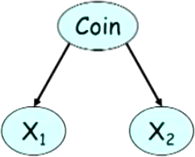
\includegraphics[width=2in]{graphics/example_coin.png}
\caption{A fair or biased coin is tossed twice. $X_1$ and $X_2$ are the two outcomes, respectively.}
\label{fig:example_coin}
\end{figure}

% C --> X_1, X_2.

$\Pr(X_2 = \text{head} | X_1 = \text{head}) > 0.5$ because the coin might not be fair.
However, $\Pr(X_2 = \text{head}| C = \text{fair coin})$ is independent of $X_1$!

Also $\Pr(X_2 = \text{head}| C = \text{biased coin})$ is independent of $X_1$. That is, once we know what the coin is, the two outcomes are no longer correlated.

In her notation,
\begin{itemize}
  \item $\Pr$ does NOT satisfy $X_1 \bot X_2$
  \item $\Pr$ satisfies $(X_1 \bot X_2 | C)$.
\end{itemize}
Conditioning can remove independence.


\paragraph{Example 2} 
We have,
\begin{equation*}
I \rightarrow G, S
\end{equation*}

\begin{equation*}
  \Pr(S, G | I=i^0) = \Pr(S | I=i^0) \Pr(G | I=i^0) \, .
\end{equation*}



\paragraph{Example 3} However, conditioning can also introduce independence.
We have,
\begin{equation*}
I, D \rightarrow G
\end{equation*}

Look at $\Pr(I, D| G = 1)$.  It couples $I$ and $D$.


\subsubsection{Independencies in Bayesian Networks}
$X$ and $Y$ are $d$-separated if $\mathbb{G}$ given $Z$,
$\text{d-sep}_{\mathbb{G}}(X, Y|Z)$,
if there is no active trail in $\mathbb{G}$ between $X$
and $Y$ given $Z$.

If $\Pr$ factorizes over $\mathbb{G}$, and $d-\text{sep}_{\mathbb{G}}(X, Y|Z)$, then $\Pr$ satisfies $(X \bot Y | Z)$.
In other words,
\begin{equation*}
  \text{factorization} \rightarrow \text{independence}
\end{equation*}

Any node is $d$-separated from its non-descendants given its parents.
In other words, if $\Pr$ factorizes over $\mathbb{G}$, then in $\Pr$,
any variable is independent of its non-descendants given its parents.


\paragraph{$I$-map (Independency Map)}

\begin{equation*}
  I(\mathbb{G}) = \{ (X \bot Y | Z) : d-\text{sep}_{\mathbb{G}}(X, Y|Z) \}
\end{equation*}

If $\Pr$ satisfies $I(\mathbb{G})$, $\mathbb{G}$ is an $I$-map of $\Pr$.

$\Pr$ factorizes over $\mathbb{G} \leftrightarrow \mathbb{G}$ is an $I$-map for $\Pr$.

\paragraph{Quiz}

$I$-maps can also be defined directly on graphs as follows. Let $I(\mathbb{G})$ be the set of independencies encoded by a graph $\mathbb{G}$. Then $\mathbb{G}_1$ is an $I$-map for $\mathbb{G}_2$ if $I(\mathbb{G}_1) \subseteq I(\mathbb{G}_2)$.

A graph $\mathbb{K}$ is an $I$-map for a graph $\mathbb{G}$ if and only if all of the independencies encoded by $\mathbb{K}$ are also encoded by $\mathbb{G}$.

\subsubsection{Naive Bayes}

Class $C \rightarrow$ Features $X_1, \ldots, X_n$.

Assume that $(X_i \bot X_j | C)$ for all $X_i, X_j$.
\begin{equation*}
  \Pr(C, X_1, \ldots, X_n) = \Pr(C) \sum_{i=1}^n \Pr(X_i | C)
\end{equation*}



\end{document}
